\documentclass{standalone}
\usepackage{tikz}
\usetikzlibrary{patterns, positioning}


\begin{document}
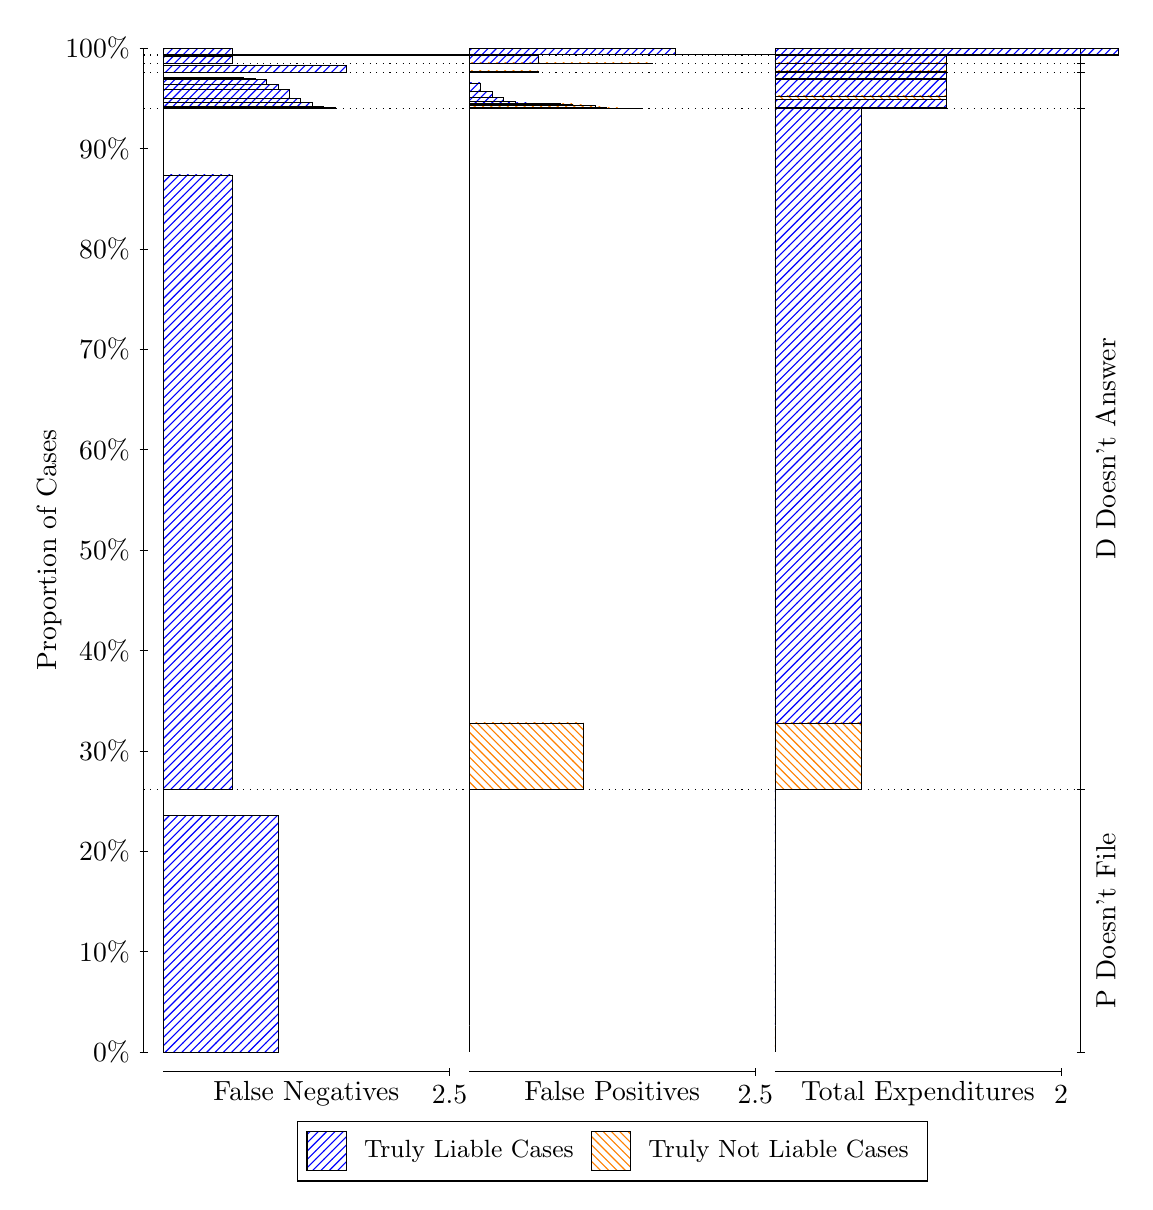
\begin{tikzpicture}
\draw[black, very thin] (1.5,1.75) -- (1.5,14.5);
\node[rotate=90, text=black, anchor=center] at (0.3, 8.125) {Proportion of Cases};
\draw[black, very thin] (1.45,1.75) -- (1.55,1.75);
\node[text=black, anchor=east] at (1.45, 1.75) {0\%};
\draw[black, very thin] (1.45,3.025) -- (1.55,3.025);
\node[text=black, anchor=east] at (1.45, 3.025) {10\%};
\draw[black, very thin] (1.45,4.3) -- (1.55,4.3);
\node[text=black, anchor=east] at (1.45, 4.3) {20\%};
\draw[black, very thin] (1.45,5.575) -- (1.55,5.575);
\node[text=black, anchor=east] at (1.45, 5.575) {30\%};
\draw[black, very thin] (1.45,6.85) -- (1.55,6.85);
\node[text=black, anchor=east] at (1.45, 6.85) {40\%};
\draw[black, very thin] (1.45,8.125) -- (1.55,8.125);
\node[text=black, anchor=east] at (1.45, 8.125) {50\%};
\draw[black, very thin] (1.45,9.4) -- (1.55,9.4);
\node[text=black, anchor=east] at (1.45, 9.4) {60\%};
\draw[black, very thin] (1.45,10.675) -- (1.55,10.675);
\node[text=black, anchor=east] at (1.45, 10.675) {70\%};
\draw[black, very thin] (1.45,11.95) -- (1.55,11.95);
\node[text=black, anchor=east] at (1.45, 11.95) {80\%};
\draw[black, very thin] (1.45,13.225) -- (1.55,13.225);
\node[text=black, anchor=east] at (1.45, 13.225) {90\%};
\draw[black, very thin] (1.45,14.5) -- (1.55,14.5);
\node[text=black, anchor=east] at (1.45, 14.5) {100\%};

\draw[black, very thin] (13.4,1.75) -- (13.4,14.5);
\draw[black, very thin] (13.35,1.75) -- (13.45,1.75);
\node[anchor=west] at (13.35, 1.75) {};
\draw[black, very thin] (13.35,5.0855) -- (13.45,5.0855);
\node[anchor=west] at (13.35, 5.0855) {};
\draw[black, very thin] (13.35,13.732) -- (13.45,13.732);
\node[anchor=west] at (13.35, 13.732) {};
\draw[black, very thin] (13.35,14.188) -- (13.45,14.188);
\node[anchor=west] at (13.35, 14.188) {};
\draw[black, very thin] (13.35,14.302) -- (13.45,14.302);
\node[anchor=west] at (13.35, 14.302) {};
\draw[black, very thin] (13.35,14.404) -- (13.45,14.404);
\node[anchor=west] at (13.35, 14.404) {};
\draw[black, very thin] (13.35,14.422) -- (13.45,14.422);
\node[anchor=west] at (13.35, 14.422) {};
\draw[black, very thin] (13.35,14.5) -- (13.45,14.5);
\node[anchor=west] at (13.35, 14.5) {};

\draw[black, very thin, pattern color=blue, pattern=north east lines] (1.75,1.75) rectangle (3.2033,4.7519);
\draw[black, very thin, pattern color=orange, pattern=north west lines] (1.75,4.7519) rectangle (1.75,5.0855);
\draw[black, very thin, pattern color=blue, pattern=north east lines] (1.75,5.0855) rectangle (2.622,12.888);
\draw[black, very thin, pattern color=orange, pattern=north west lines] (1.75,12.888) rectangle (1.75,13.732);
\draw[black, very thin, pattern color=blue, pattern=north east lines] (1.75,13.732) rectangle (3.93,13.746);
\draw[black, very thin, pattern color=blue, pattern=north east lines] (1.75,13.746) rectangle (3.7847,13.755);
\draw[black, very thin, pattern color=blue, pattern=north east lines] (1.75,13.755) rectangle (3.6393,13.806);
\draw[black, very thin, pattern color=blue, pattern=north east lines] (1.75,13.806) rectangle (3.494,13.864);
\draw[black, very thin, pattern color=blue, pattern=north east lines] (1.75,13.864) rectangle (3.3487,13.97);
\draw[black, very thin, pattern color=blue, pattern=north east lines] (1.75,13.97) rectangle (3.2033,14.042);
\draw[black, very thin, pattern color=blue, pattern=north east lines] (1.75,14.042) rectangle (3.058,14.099);
\draw[black, very thin, pattern color=blue, pattern=north east lines] (1.75,14.099) rectangle (2.9127,14.117);
\draw[black, very thin, pattern color=blue, pattern=north east lines] (1.75,14.117) rectangle (2.7673,14.127);
\draw[black, very thin, pattern color=orange, pattern=north west lines] (1.75,14.127) rectangle (1.75,14.188);
\draw[black, very thin, pattern color=blue, pattern=north east lines] (1.75,14.188) rectangle (4.0753,14.279);
\draw[black, very thin, pattern color=orange, pattern=north west lines] (1.75,14.279) rectangle (1.75,14.302);
\draw[black, very thin, pattern color=blue, pattern=north east lines] (1.75,14.302) rectangle (2.622,14.397);
\draw[black, very thin, pattern color=orange, pattern=north west lines] (1.75,14.397) rectangle (1.75,14.404);
\draw[black, very thin, pattern color=blue, pattern=north east lines] (1.75,14.404) rectangle (5.8193,14.418);
\draw[black, very thin, pattern color=orange, pattern=north west lines] (1.75,14.418) rectangle (1.75,14.422);
\draw[black, very thin, pattern color=blue, pattern=north east lines] (1.75,14.422) rectangle (2.622,14.498);
\draw[black, very thin, pattern color=orange, pattern=north west lines] (1.75,14.498) rectangle (1.75,14.5);
\draw[black, very thin, pattern color=orange, pattern=north west lines] (5.6333,1.75) rectangle (5.6333,2.0835);
\draw[black, very thin, pattern color=blue, pattern=north east lines] (5.6333,2.0835) rectangle (5.6333,5.0855);
\draw[black, very thin, pattern color=orange, pattern=north west lines] (5.6333,5.0855) rectangle (7.0867,5.9296);
\draw[black, very thin, pattern color=blue, pattern=north east lines] (5.6333,5.9296) rectangle (5.6333,13.732);
\draw[black, very thin, pattern color=orange, pattern=north west lines] (5.6333,13.732) rectangle (7.8133,13.734);
\draw[black, very thin, pattern color=orange, pattern=north west lines] (5.6333,13.734) rectangle (7.668,13.735);
\draw[black, very thin, pattern color=orange, pattern=north west lines] (5.6333,13.735) rectangle (7.5227,13.741);
\draw[black, very thin, pattern color=orange, pattern=north west lines] (5.6333,13.741) rectangle (7.3773,13.753);
\draw[black, very thin, pattern color=orange, pattern=north west lines] (5.6333,13.753) rectangle (7.232,13.768);
\draw[black, very thin, pattern color=orange, pattern=north west lines] (5.6333,13.768) rectangle (7.0867,13.778);
\draw[black, very thin, pattern color=orange, pattern=north west lines] (5.6333,13.778) rectangle (6.9413,13.79);
\draw[black, very thin, pattern color=orange, pattern=north west lines] (5.6333,13.79) rectangle (6.796,13.792);
\draw[black, very thin, pattern color=orange, pattern=north west lines] (5.6333,13.792) rectangle (6.6507,13.794);
\draw[black, very thin, pattern color=blue, pattern=north east lines] (5.6333,13.794) rectangle (6.36,13.803);
\draw[black, very thin, pattern color=blue, pattern=north east lines] (5.6333,13.803) rectangle (6.2147,13.821);
\draw[black, very thin, pattern color=blue, pattern=north east lines] (5.6333,13.821) rectangle (6.0693,13.878);
\draw[black, very thin, pattern color=blue, pattern=north east lines] (5.6333,13.878) rectangle (5.924,13.951);
\draw[black, very thin, pattern color=blue, pattern=north east lines] (5.6333,13.951) rectangle (5.7787,14.056);
\draw[black, very thin, pattern color=blue, pattern=north east lines] (5.6333,14.056) rectangle (5.6333,14.188);
\draw[black, very thin, pattern color=orange, pattern=north west lines] (5.6333,14.188) rectangle (6.5053,14.211);
\draw[black, very thin, pattern color=blue, pattern=north east lines] (5.6333,14.211) rectangle (5.6333,14.302);
\draw[black, very thin, pattern color=orange, pattern=north west lines] (5.6333,14.302) rectangle (7.9587,14.31);
\draw[black, very thin, pattern color=blue, pattern=north east lines] (5.6333,14.31) rectangle (6.5053,14.404);
\draw[black, very thin, pattern color=orange, pattern=north west lines] (5.6333,14.404) rectangle (6.5053,14.408);
\draw[black, very thin, pattern color=blue, pattern=north east lines] (5.6333,14.408) rectangle (5.6333,14.422);
\draw[black, very thin, pattern color=orange, pattern=north west lines] (5.6333,14.422) rectangle (9.7027,14.423);
\draw[black, very thin, pattern color=blue, pattern=north east lines] (5.6333,14.423) rectangle (8.2493,14.5);
\draw[black, very thin, pattern color=orange, pattern=north west lines] (9.5167,1.75) rectangle (9.5167,2.0835);
\draw[black, very thin, pattern color=blue, pattern=north east lines] (9.5167,2.0835) rectangle (9.5167,5.0855);
\draw[black, very thin, pattern color=orange, pattern=north west lines] (9.5167,5.0855) rectangle (10.607,5.9296);
\draw[black, very thin, pattern color=blue, pattern=north east lines] (9.5167,5.9296) rectangle (10.607,13.732);
\draw[black, very thin, pattern color=orange, pattern=north west lines] (9.5167,13.732) rectangle (11.697,13.747);
\draw[black, very thin, pattern color=blue, pattern=north east lines] (9.5167,13.747) rectangle (11.697,13.852);
\draw[black, very thin, pattern color=orange, pattern=north west lines] (9.5167,13.852) rectangle (11.697,13.892);
\draw[black, very thin, pattern color=blue, pattern=north east lines] (9.5167,13.892) rectangle (11.697,14.106);
\draw[black, very thin, pattern color=orange, pattern=north west lines] (9.5167,14.106) rectangle (11.697,14.113);
\draw[black, very thin, pattern color=blue, pattern=north east lines] (9.5167,14.113) rectangle (11.697,14.188);
\draw[black, very thin, pattern color=orange, pattern=north west lines] (9.5167,14.188) rectangle (11.697,14.211);
\draw[black, very thin, pattern color=blue, pattern=north east lines] (9.5167,14.211) rectangle (11.697,14.302);
\draw[black, very thin, pattern color=orange, pattern=north west lines] (9.5167,14.302) rectangle (11.697,14.31);
\draw[black, very thin, pattern color=blue, pattern=north east lines] (9.5167,14.31) rectangle (11.697,14.404);
\draw[black, very thin, pattern color=orange, pattern=north west lines] (9.5167,14.404) rectangle (13.877,14.408);
\draw[black, very thin, pattern color=blue, pattern=north east lines] (9.5167,14.408) rectangle (13.877,14.422);
\draw[black, very thin, pattern color=orange, pattern=north west lines] (9.5167,14.422) rectangle (13.877,14.423);
\draw[black, very thin, pattern color=blue, pattern=north east lines] (9.5167,14.423) rectangle (13.877,14.5);
\draw[black, dotted] (1.5,5.0855) -- (13.4,5.0855);
\draw[black, dotted] (1.5,13.732) -- (13.4,13.732);
\draw[black, dotted] (1.5,14.188) -- (13.4,14.188);
\draw[black, dotted] (1.5,14.302) -- (13.4,14.302);
\draw[black, dotted] (1.5,14.404) -- (13.4,14.404);
\draw[black, dotted] (1.5,14.422) -- (13.4,14.422);
\draw[black, very thin] (1.75,1.5) -- (5.3833,1.5);
\node[text=black, anchor=north] at (3.5667, 1.5) {False Negatives};
\draw[black, very thin] (5.3833,1.45) -- (5.3833,1.55);
\node[text=black, anchor=north] at (5.3833, 1.45) {2.5};

\draw[black, very thin] (5.6333,1.5) -- (9.2667,1.5);
\node[text=black, anchor=north] at (7.45, 1.5) {False Positives};
\draw[black, very thin] (9.2667,1.45) -- (9.2667,1.55);
\node[text=black, anchor=north] at (9.2667, 1.45) {2.5};

\draw[black, very thin] (9.5167,1.5) -- (13.15,1.5);
\node[text=black, anchor=north] at (11.333, 1.5) {Total Expenditures};
\draw[black, very thin] (13.15,1.45) -- (13.15,1.55);
\node[text=black, anchor=north] at (13.15, 1.45) {2};

\node[text=black, centered, rotate=90] at (13.72, 3.4177) {P Doesn't File};
\node[text=black, centered, rotate=90] at (13.72, 9.409) {D Doesn't Answer};






\draw (7.449999999999999,1.5) node[draw=none] (baseCoordinate) {};
\begin{scope}[align=center]
        \matrix[scale=0.5, draw=black, below=0.5cm of baseCoordinate, nodes={draw}, column sep=0.1cm]{
            \node[rectangle, draw, minimum width=0.5cm, minimum height=0.5cm, pattern color=blue, pattern=north east lines] {}; &
            \node[draw=none, font=\small, text=black] (B) {Truly Liable Cases}; &
            \node[rectangle, draw, minimum width=0.5cm, minimum height=0.5cm, pattern color=orange, pattern=north west lines] {}; &
            \node[draw=none, font=\small, text=black] (B) {Truly Not Liable Cases}; \\
            };
\end{scope}

\end{tikzpicture}
\end{document}